\documentclass[a4paper,12pt]{article}
\usepackage{mathtools,amsfonts,amssymb,amsmath, bm,commath,multicol}
\usepackage{algorithmicx, tkz-graph, algorithm, fancyhdr, pgfplots}
\usepackage{fancyvrb}

\usepackage[noend]{algpseudocode}

\pagestyle{fancy}
\fancyhf{}
\rhead{13/3/2017 ::: Nandan Rao}
\lhead{Machine Learning ::: Problemset 3}
\rfoot{\thepage}


\DefineVerbatimEnvironment{juliaout}{Verbatim}{}
\DefineVerbatimEnvironment{juliacode}{Verbatim}{fontshape=sl, fontsize=\tiny}
\DefineVerbatimEnvironment{juliaterm}{Verbatim}{}


\begin{document}

\section*{Problem 13}
We begin with the naive solution, writing down our most explicit objective:

\begin{align*}
\text{Maximize }  &\null \gamma  \\
\text{s.t. } &\null  \frac{y_iw^Tx_i}{||w||} \geq \gamma
\end{align*}
%
We observe that the scaling factor $||w||$ could instead be applied directly to $\gamma$:
w\begin{align*}
\text{Maximize }  &\null \frac{\gamma}{||w||}  \\
\text{s.t. } &\null  y_iw^Tx_i \geq \gamma
\end{align*}
%
Which brings us nicely to the realization that we could remove $\gamma$ altogether, replacing it with with a constant, and focus intead on maximizing only the scaling factor $\frac{1}{||w||}$, or conversely minimizing the norm:
\begin{align*}
\text{Minimize }  &\null ||w||^2  \\
\text{s.t. } &\null  y_iw^Tx_i \geq 1
\end{align*}
%
We solve the Lagrangian duel, imposing lagrangian multipliers $\alpha$ for each point to constrain them on the correct side of the margins. The dual and the solution:
\begin{align*}
\text{Maximize}  &\null \sum_i^n \alpha_i - \frac{1}{2}\sum_{i,j}^n y_iy_j\alpha_i \alpha_j x_i^Tx_j\\
\text{s.t. } &\null  \alpha_i \geq 0 \\
  &\null \sum_{i}^n\alpha_iy_i = 0
\end{align*}
Here we see the curious fact of the support vectors. The constraints in their lagrangian form ($\alpha$) will only be active, naturally, for the data points which lie on the margin. Everything else will not need any constraints, and hence the $\alpha$ corresponding to that point will be zero. This is to say that our final $w*$ is defined by the following portion of our objective function:
\begin{align*}
\sum_{i,j \in S}^n y_iy_j\alpha_i \alpha_j x_i^Tx_j\\
\end{align*}
%
Where S is the set of points which lie on the margins. It is clear to see here that this is a linear product of scalar products of all the data points in S, hence, within the vector space spanned by those points.
\section*{Problem 14}

\subsubsection*{Kernel Function}

\begin{align*}
K(x,y) &= \langle \Phi(x), \Phi(y) \rangle \\
K(x,y) &= \sum_{n=0}^{\infty} \frac{1}{\sqrt{n!}}x^ne^{-x^2/2}\frac{1}{\sqrt{n!}}y^ne^{-y^2/2} \\
K(x,y) &= e^{-x^2/2}e^{-y^2/2} \sum_{n=0}^{\infty} \frac{1}{n!}(xy)^n \\
K(x,y) &=  e^{-x^2/2}e^{-y^2/2}e^{xy} \\
K(x,y) &=  e^{xy - x^2/2 -y^2/2} \\
K(x,y) &=  e^{\frac{1}{2}(x - y)(y - x)} \\
K(x,y) &=  e^{- \frac{1}{2}(x - y)^2}
\end{align*}

\subsubsection*{Kernel in $\mathbb{R}^d$}
Recognizing gaussianity when we see it, an easy choice is the multivariate flavor:
\begin{align*}
K(X,Y) &=  e^{- \frac{1}{2}(X - Y)^T(X - Y)}
\end{align*}

\subsubsection*{Corresponding Feature Map}

We begin by rewriting our Kernel function:
\begin{align*}
K(X,Y) &=  e^{X^TY - ||X||^2/2 - ||Y||^2/2}
\end{align*}
%
This allows us to more easily see the component parts:
\begin{align*}
\Phi(X) &= \frac{1}{\sqrt{n!}}||X||^n e^{-\frac{1}{2}||X||^2}
\end{align*}

\section*{Problem 15}

\subsubsection*{Product of Two Kernels}

\begin{align*}
K_1K_2 &= \langle \Phi_1(x), \Phi_1(y) \rangle \langle \Phi_2(x), \Phi_2(y) \rangle \\
K_1K_2 &= \sum_{i=0}^{\infty} \Phi_1(x)_i\Phi_1(y)_i \sum_{j=0}^{\infty} \Phi_2(x)_j\Phi_2(y)_j \\
K_1K_2 &= \sum_{i=0}^{\infty} \sum_{j=0}^{\infty} \Phi_1(x)_i\Phi_1(y)_i\Phi_2(x)_j\Phi_2(y)_j
\end{align*}
We can therefore define a new feature map:
\begin{align*}
\Phi_3(x) &= \Phi_i(x) \sum_{j=0}^{\infty} \Phi_j(x)
\end{align*}
And we have a scalar product:
\begin{align*}
K_1K_2 &= \sum_{i=0}^{\infty} \Phi_3(x)_i\Phi_3(y)_i \\
K_1K_2 &= \langle \Phi_3(x), \Phi_3(y) \rangle
\end{align*}

\subsubsection*{Sum of Two Kernels}

\begin{align*}
K_1 + K_2 &= \langle \Phi_1(x), \Phi_1(y) \rangle + \langle \Phi_2(x), \Phi_2(y) \rangle \\
K_1 + K_2 &= \sum_{i=0}^{\infty} \Phi_1(x)_i\Phi_1(y)_i + \sum_{j=0}^{\infty} \Phi_2(x)_j\Phi_2(y)_j
\end{align*}
Here we see that this is simply the inner product of the two vectors concatenated together, so the corresponding new feature map can be defined as such, proving that this is indeed a valid kernel:
\begin{align*}
\Phi_3(x) &= \big[ \Phi_1(x) \ \Phi_2(x) \big]
\end{align*}

\section*{Problem 16}




\subsection*{Small Sample Sizes}

We beging by comparing how, especially on low number of training examples, the standard tree is prone to overfitting, especially with more depth, while the bagged quorum performs much better despite the expremely small sample size. (Test size is the sample as training size).

\subsubsection*{Standard Tree, n = 20}
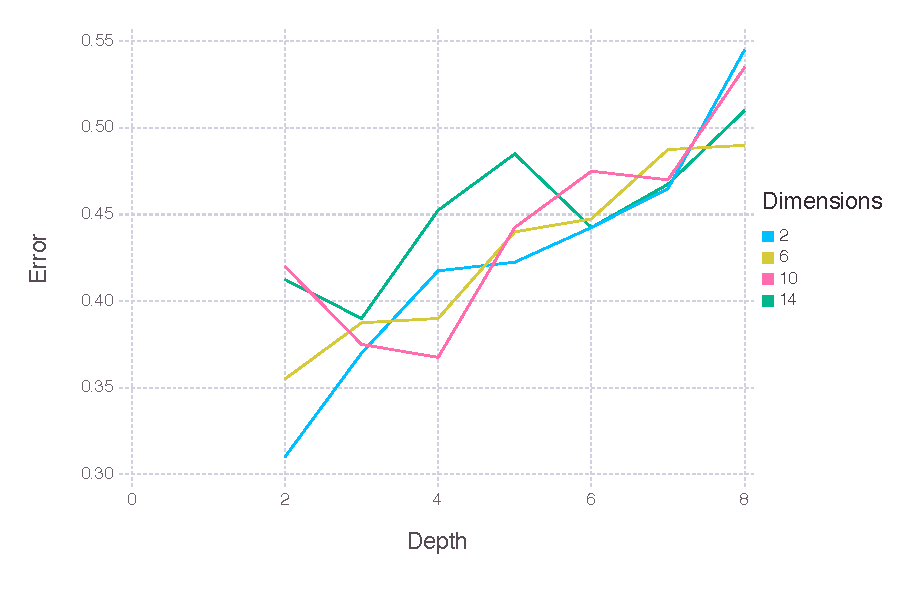
\includegraphics[width=\linewidth]{figures/problemset_2_1.pdf}



\subsubsection*{Bagged Trees, n = 20}
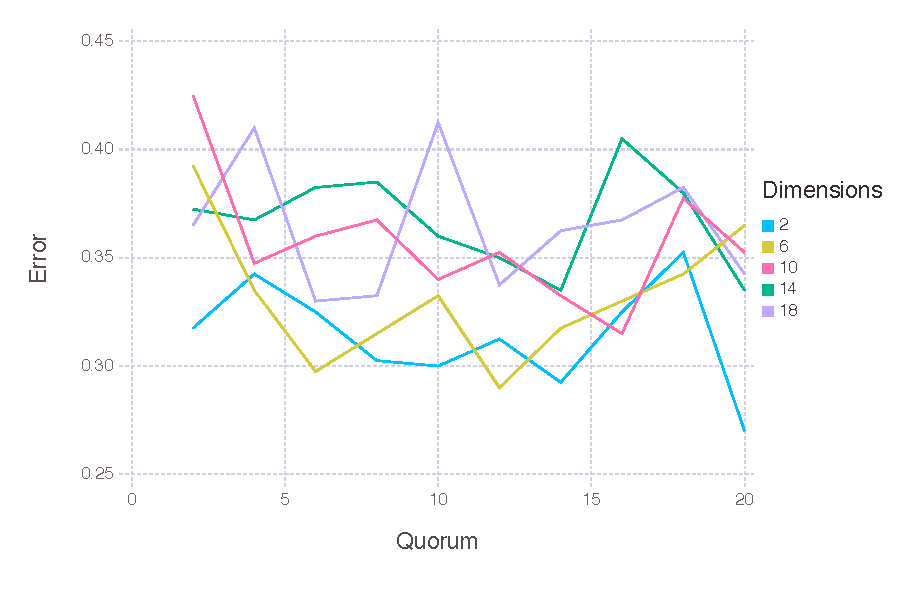
\includegraphics[width=\linewidth]{figures/problemset_3_1.pdf}



\subsection*{Larger Sample Sizes}
The most interesting thing to see here is that the subsampling will perform worse and worse with greater dimensions. This is natural, as our data only has information in the first couple of dimensions! Naturally, in two dimensions, then, the subsampling works ok. The bagging is also still outperforming the standard results, although you see the standard tree with low depth does alright, which makes sense, as the sample size increases this unbiased estimator decreases the variance and therefore improves!

\subsubsection*{Subsampled Trees, n = 200}
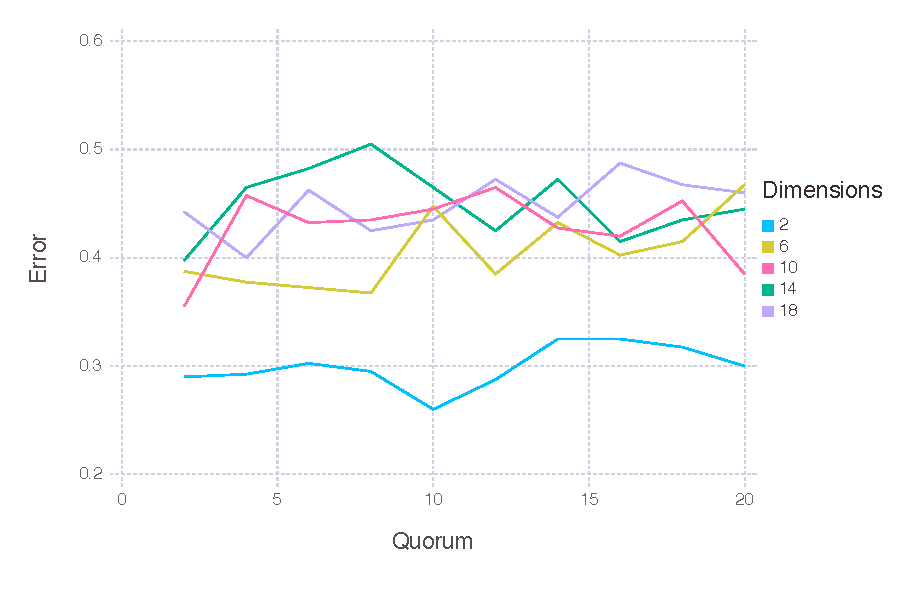
\includegraphics[width=\linewidth]{figures/problemset_4_1.pdf}



\subsubsection*{Standard Trees, n = 200}
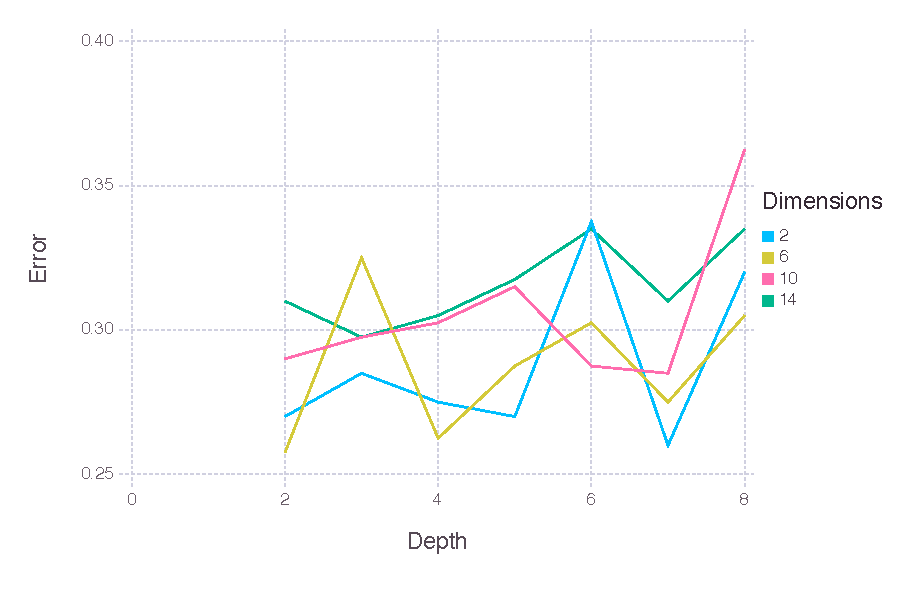
\includegraphics[width=\linewidth]{figures/problemset_5_1.pdf}



\subsubsection*{Bagged Trees, n = 200}
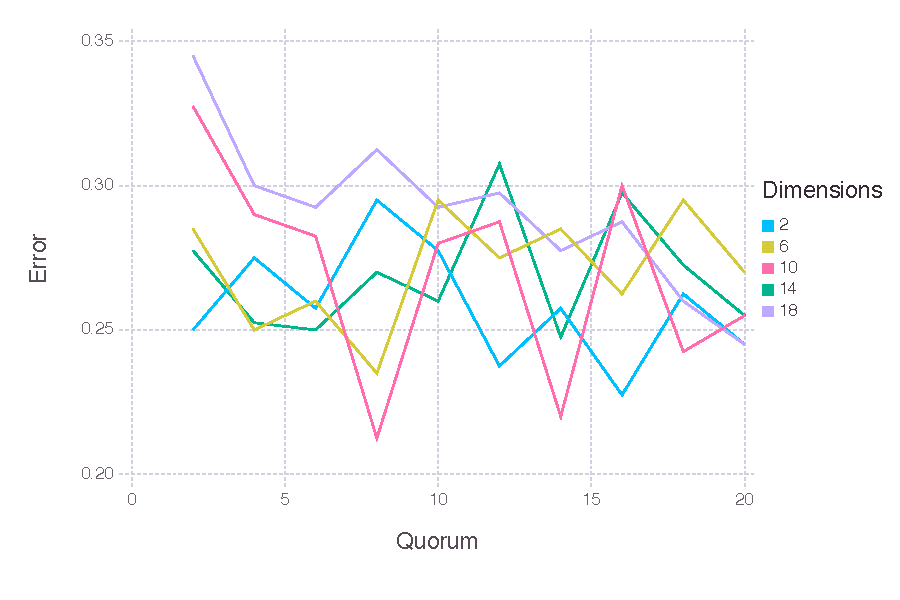
\includegraphics[width=\linewidth]{figures/problemset_6_1.pdf}








\section*{Code}

\begin{juliacode}
using Distributions
using DataFrames
using Gadfly
using Base.Test

function tuples_to_data(a)
    if length(a) == 0
        return Dict(:X => [], :y => [])
    end
    X = reduce(vcat, [t[1]' for t in a])
    y  = [t[2] for t in a]
    Dict(:X => X, :y => y)
end

make_tuples(X, y) = [(X[i,:],y) for i in 1:size(X)[1]]

function make_ones(N, d)
    m = append!(ones(2), fill(0, d - 2))
    rand(MvNormal(m, 1), N)'
end

function make_zeros(N, d)
    m = zeros(d)
    rand(MvNormal(m, 1), N)'
end

function generate_distributions(N, d = 5)
    o = make_ones(Int(N/2), d)
    z = make_zeros(Int(N/2), d)
    vcat(make_tuples(o, 1), make_tuples(z,0))
end

function ent(targets)
    if length(targets) == 0
        return 0
    end
    probs = [count(t -> t == class, targets)/length(targets) for class in unique(targets)]
    sum([p*log(2, 1/p) for p in probs])
end

function counter(a, b, class)
    prev = a[end]
    d = b[2] == class ?
        Dict(:a => prev[:a] - 1) :
        Dict(:b => prev[:b] + 1)
    vcat(a, [merge(prev, d)])
end


make_counter(class) = (a,b) -> counter(a,b,class)

function find_threshold(x, y, class)
    vals = collect(zip(x,y))
    N_class = count(t -> t == class, y)
    a = reduce(make_counter(class), [Dict(:a => N_class, :b => 0)], vals)
    scores = [sum(values(d)) for d in a]
    sortperm(scores)[1], minimum(scores)
end


function info_gain(a, b)
    y = vcat(a,b)
    prob(s) = length(s)/length(y)
    new_ent = sum([prob(s) * ent(s) for s in [a,b]])
    ent(y) - new_ent
end

function sort_and_get_feature(data, i)
    x = data[:X][:,i]
    y = data[:y]
    vals = sort(collect(zip(x, y)), by = t -> t[1])
    [t[1] for t in vals], [t[2] for t in vals]
end

function thresh_value(x, y, i)
    # Check from left-right against both class types
    o = find_threshold(x, y, 1)
    z = find_threshold(x, y, 0)
    # ones are left, zeros is right! rename???
    if o[2] == z[2]
        thresh,a,b = o[1] < z[1] ? (o[1],:left, :right) : (z[1],:right,:left)
    else
        thresh,a,b = o[2] < z[2] ? (o[1],:left, :right) : (z[1],:right,:left)
    end
    val = thresh > 1 ? (x[thresh-1] + x[thresh])/2 : x[thresh]
    val, a, b
end

function make_fn(x, y, i)
    # function expects a single data point, checks the feature,
    # and returns left or right based on split
    val,a,b = thresh_value(x, y, i)
    z -> z[i] <= val ? a : b
end


function splitter(data, i)
    x,y = sort_and_get_feature(data, i)
    make_fn(x,y,i)
end

function make_fns(data)
    d = size(data[:X])[2]
    [splitter(data, i) for i in 1:d]
end


function split_data_by_fn(data, fn)
    X = data[:X]
    y = data[:y]
    N = size(X)[1]
    dirs = [fn(X[i,:]) for i in 1:N]
    left = [(X[i,:],y[i]) for i in 1:N if dirs[i] == :left]
    right = [(X[i,:],y[i]) for i in 1:N if dirs[i] == :right]
    tuples_to_data(left), tuples_to_data(right)
end

function find_next_split(data)
    fns = make_fns(data)
    splits = [split_data_by_fn(data, fn) for fn in fns]
    infos = [info_gain(a[:y], b[:y]) for (a,b) in splits]
    i = indmax(infos)
    fns[i], splits[i][1], splits[i][2]
end

leaf(c) = Dict(:class => c)
make_leaf(y) = leaf(Int(round(mean(y))))

function build_tree(data, k)
    # Stop if we've reached max Depth.
    if k == 0
        return make_leaf(data[:y])
    end
    fn, left, right = find_next_split(data)
    # Stop also if we have a one-sided split
    if isempty(left[:y])
        return leaf(0)
    elseif isempty(right[:y])
        return leaf(1)
    end
    # Else recurse!
    Dict(:fn => fn,
         :left => build_tree(left, k-1),
         :right => build_tree(right, k-1))
end

function classifier(x, node)
    if haskey(node,:class)
        return node[:class]
    end
    dir = node[:fn](x)
    classifier(x, node[dir]) # recur
end

function make_basic_classifier(tuples, k, S)
    tree = build_tree(tuples_to_data(tuples), k)
    x -> classifier(x, tree)
end

function bagged_trees(tuples, k, S)
    N = length(tuples)
    new_tuples = [getindex(tuples, rand(1:N, N)) for s in 1:S]
    sets = [tuples_to_data(s) for s in new_tuples]
    [build_tree(d, k) for d in sets]
end

vote(classifiers, x) = Int(round(mean([c(x) for c in classifiers])))

function make_bagged_classifiers(tuples, k, S)
    trees = bagged_trees(tuples, k, S)
    classifiers = [x -> classifier(x, t) for t in trees]
    x -> vote(classifiers, x)
end

subsample(data, cols) = Dict(:X => data[:X][:,cols], :y => data[:y])

function subsampling_classifier(data, k, c = 2)
    dims = size(data[:X])[2]
    cols = rand(1:dims, 2)
    tree = build_tree(subsample(data, cols), k)
    x -> classifier(x[cols], tree)
end

function make_subsampling_classifiers(tuples, k, S)
    data = tuples_to_data(tuples)
    classifiers = [subsampling_classifier(data, k) for i in S]
    x -> vote(classifiers, x)
end

function test_classifiers(N, d, k, t, S, fn)
    tuples = generate_distributions(N, d)
    tests = generate_distributions(t, d)
    cl = fn(tuples, k, S)
    mean([y == cl(x) ? 0 : 1 for (x,y) in tests])
end

runner(N,d,k,t,S,fn,m) = mean([test_classifiers(N, d, k, t, S, fn) for i in 1:m])

function plot_standard(N, t, m, D = 2:4:18, K = 2:1:8)
    make_frame(v,d,k) = DataFrame(Error = v, Dimensions = string(d), Depth = k)
    d = vcat([make_frame(runner(N, d, k, t, 1, make_basic_classifier, m), d, k) for d in D for k in K])
    plot(d, x = :Depth, y = :Error, color = :Dimensions, Geom.line)
end

function plot_bagged(N, t, m, k = 2, D = 2:4:18, Q = 2:2:20)
    make_frame(v,d,q) = DataFrame(Error = v, Dimensions = string(d), Quorum = q)
    d = vcat([make_frame(runner(N, d, k, t, q, make_bagged_classifiers, m), d, q) for d in D for q in Q])
    plot(d, x = :Quorum, y = :Error, color = :Dimensions, Geom.line)
end

function plot_subsampling(N, t, m, k = 2, D = 2:4:18, Q = 2:2:20)
    make_frame(v,d,q) = DataFrame(Error = v, Dimensions = string(d), Quorum = q)
    d = vcat([make_frame(runner(N, d, k, t, q, make_subsampling_classifiers, m), d, q) for d in D for q in Q])
    plot(d, x = :Quorum, y = :Error, color = :Dimensions, Geom.line)
end
\end{juliacode}



\end{document}